\documentclass{article}

\usepackage{amsmath}
\usepackage{amsfonts}
\usepackage{minted}
\usepackage{ctex}
\usepackage{xeCJK}
\usepackage{graphics}
\usepackage{booktabs}
\usepackage{pgfplots}
\usepackage{authblk}
\usepackage[colorlinks,linkcolor=blue]{hyperref}

\pgfplotsset{compat=1.15}

\setCJKmainfont[ItalicFont={楷体}, BoldFont={黑体}]{宋体}


\title{rCore 中开发环境的搭建}
\author{罗崚骁\quad 宋香君}
% \author[1]{罗崚骁}
% \author[2] {宋香君}
\affil{\texttt {\{luolx17, songxj17\}@mails.tsinghua.edu.cn}}

\begin{document}
    \maketitle

    \section{课程设计目标}
    本组致力于为 rCore 增加相关的软件支持,使得 rCore 具有一定软件开发能力,为此需要对 rCore 的功能进行进一步完善,尤其是系统调用的完善。

    设想的开发环境包含的软件工具有:
    \begin{itemize}
        \item C/C++ 开发:基于 musl libc 的 gcc 工具链
        \item 工程构建:GNU make, CMake
        \item Rust 开发:rust 工具链
        \item 版本控制系统:git
        \item 编辑器:vi, vim
        \item 软件包管理器:cargo,apk
    \end{itemize}

    \section{课程设计背景}
    随着 rCore 开发团队的不懈努力,rCore 已经具备了运行一些软件的能力。但是,rCore 的软件开发能力还稍显不足,比如:
    \begin{itemize}
        \item 编译器支持不足,目前仅支持 musl-gcc
        \item C/C++,Rust 标准库实现支持不详,缺少测试,目前仅支持 musl-libc
        \item 没有版本控制系统
        \item 缺少项目构建工具
        \item 编辑器只能勉强使用(vi)
        \item 没有软件包管理器,甚至不太有从源码安装软件的能力
    \end{itemize}

    这些显然不是一个优秀的操作系统应该具有的状态,因此我们小组决定为 rCore 支持上述类型的软件使其具有软件开发的能力。

    \section{已有相关工作}
    \begin{itemize}
        \item rCore 已经实现了相当数量的系统调用,能够支持 \href{https://github.com/rcore-os/rcore-user}{rcore-user} 中的软件,
        \item 考虑到编译器是我们的课程设计中重要的一环,尤其可以参考此前 rCore 对 musl-gcc 的支持历程
        \item 可以设法获取的各种满足我们需求的开源软件,这一点决定了我们的工作思路是对 rCore 针对软件进行完善,而非针对 rCore 开发软件
    \end{itemize}

    \section{工作计划及目前进展}

    工作计划按如下顺序开展:

    \begin{itemize}
        \item 完善对 gcc 的支持,测试 C/C++ 标准库实现
        \item 支持 make,使 rCore 具备从源码安装软件的能力(除此之外,还可考虑支持 CMake)
        \item 支持 Git
        \item 支持 Rust 工具链,主要包括:
        \begin{itemize}
            \item rustc
            \item cargo
            \item 测试 rust 标准库实现
        \end{itemize}
        \item 支持更多的编辑器(nano,vim 等)
    \end{itemize}

    \section{待解决的问题}

    如果想要从源码安装软件,首先需要有执行脚本文件的能力。经测试使用 sh 命令执行脚本文件时,
    会卡在一处对 stdin 的读入上,调研


    \section{软件支持流程}
    \subsection{安装}

    由于现在还不能使用包管理器,因此如何将软件安装到 rCore 中是一个值得拿出来考虑的问题。可能尝试的途径有:
    \begin{itemize}
        \item 寻找官方发布的预编译版本(比如 musl-rust),这种做法是最方便的
        \item 下载软件源码,在外部操作系统编译好后复制到 rCore 的文件系统中
        \item 当 rCore 支持 Make 后,也可以尝试直接在 rCore 中从源码安装软件(关于这一点,受制于编译器运行速度,虽然这是我们设想的软件开发环境应该具有的一个特质,但是目前这个想法看起来很难达到较好的效果)        
    \end{itemize}

    \subsection{测试}

    软件测试似乎本来就是一个不可能做到完美的工作。受制于各方面因素,目前我们决定采用一些较为勉强的方法对 rCore 中的软件进行测试。

    \begin{itemize}
        \item 对于C/C++,Rust 标准库的测试,似乎没有找到官方公开的测例,我们决定测试以编译并运行一些具有一定规模的使用了大量标准库的工程的形式进行
        \item 对于各种软件,决定选取其重要功能进行测试,例如:
        \begin{itemize}
            \item make 是否能顺利构建项目、是否支持增量构建等
            \item Git 的 add,commit,log,status,branch 等功能
            \item 当然如果能找到测例的话就最好了
        \end{itemize}
    \end{itemize}

    需要指出的是,通常的软件测试是在给定的操作系统上测试其表现,是软件对操作系统的适应,
    而本次课程设计中是针对软件完善操作系统使操作系统能适应软件的运行。
    
    \newpage
    至于如何做到这一点,
    可以利用 rCore 的记录功能查看哪些系统调用尚未实现或实现不完全,以此来补充和调试系统
    调用的实现。

    \begin{figure}[H]
        \centering
        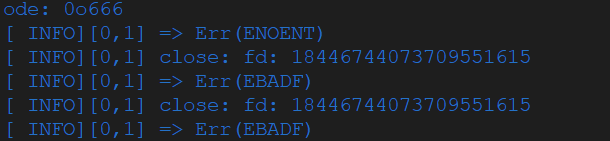
\includegraphics[width=\linewidth]{assets/syscall0.png}
        % \caption{}
        % \label{}
    \end{figure}
    \begin{figure}[H]
        \centering
        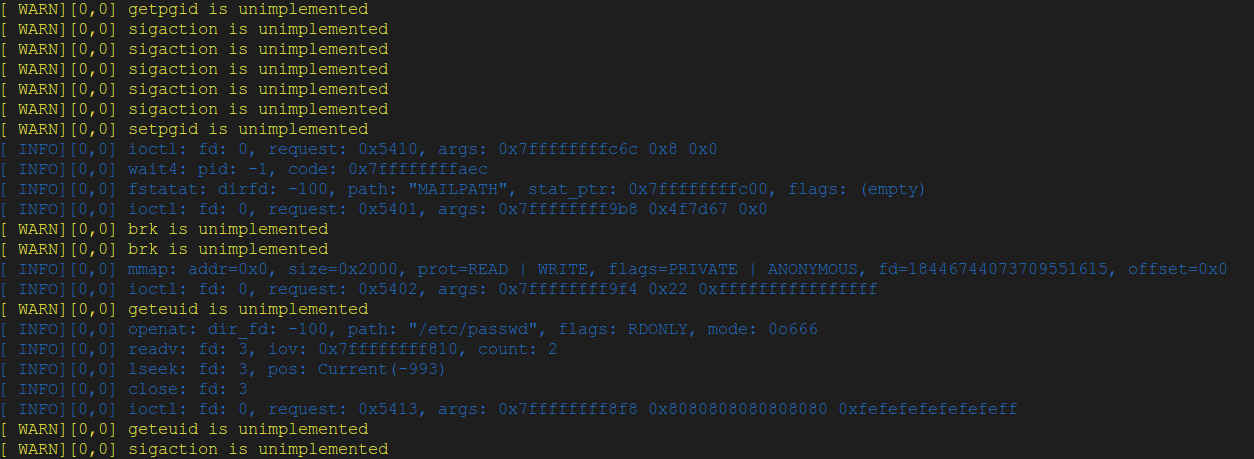
\includegraphics[width=\linewidth]{assets/syscall1.png}
        % \caption{}
        % \label{}
    \end{figure}


    \section{小组分工}
    两人都需要对各种系统调用进行实现和完善。在具体支持的软件上分工如下:
    \begin{itemize}
        \item 罗崚骁:Git,Cargo 离线版, 测试 C++ 与 Rust 项目
        \item 宋香君:make, CMake, 测试 C 项目
    \end{itemize}
\end{document}